\documentclass[usermanual/man.tex]{subfiles}
\section{Apparaten}

\begin{figure}[H]
    \centering
    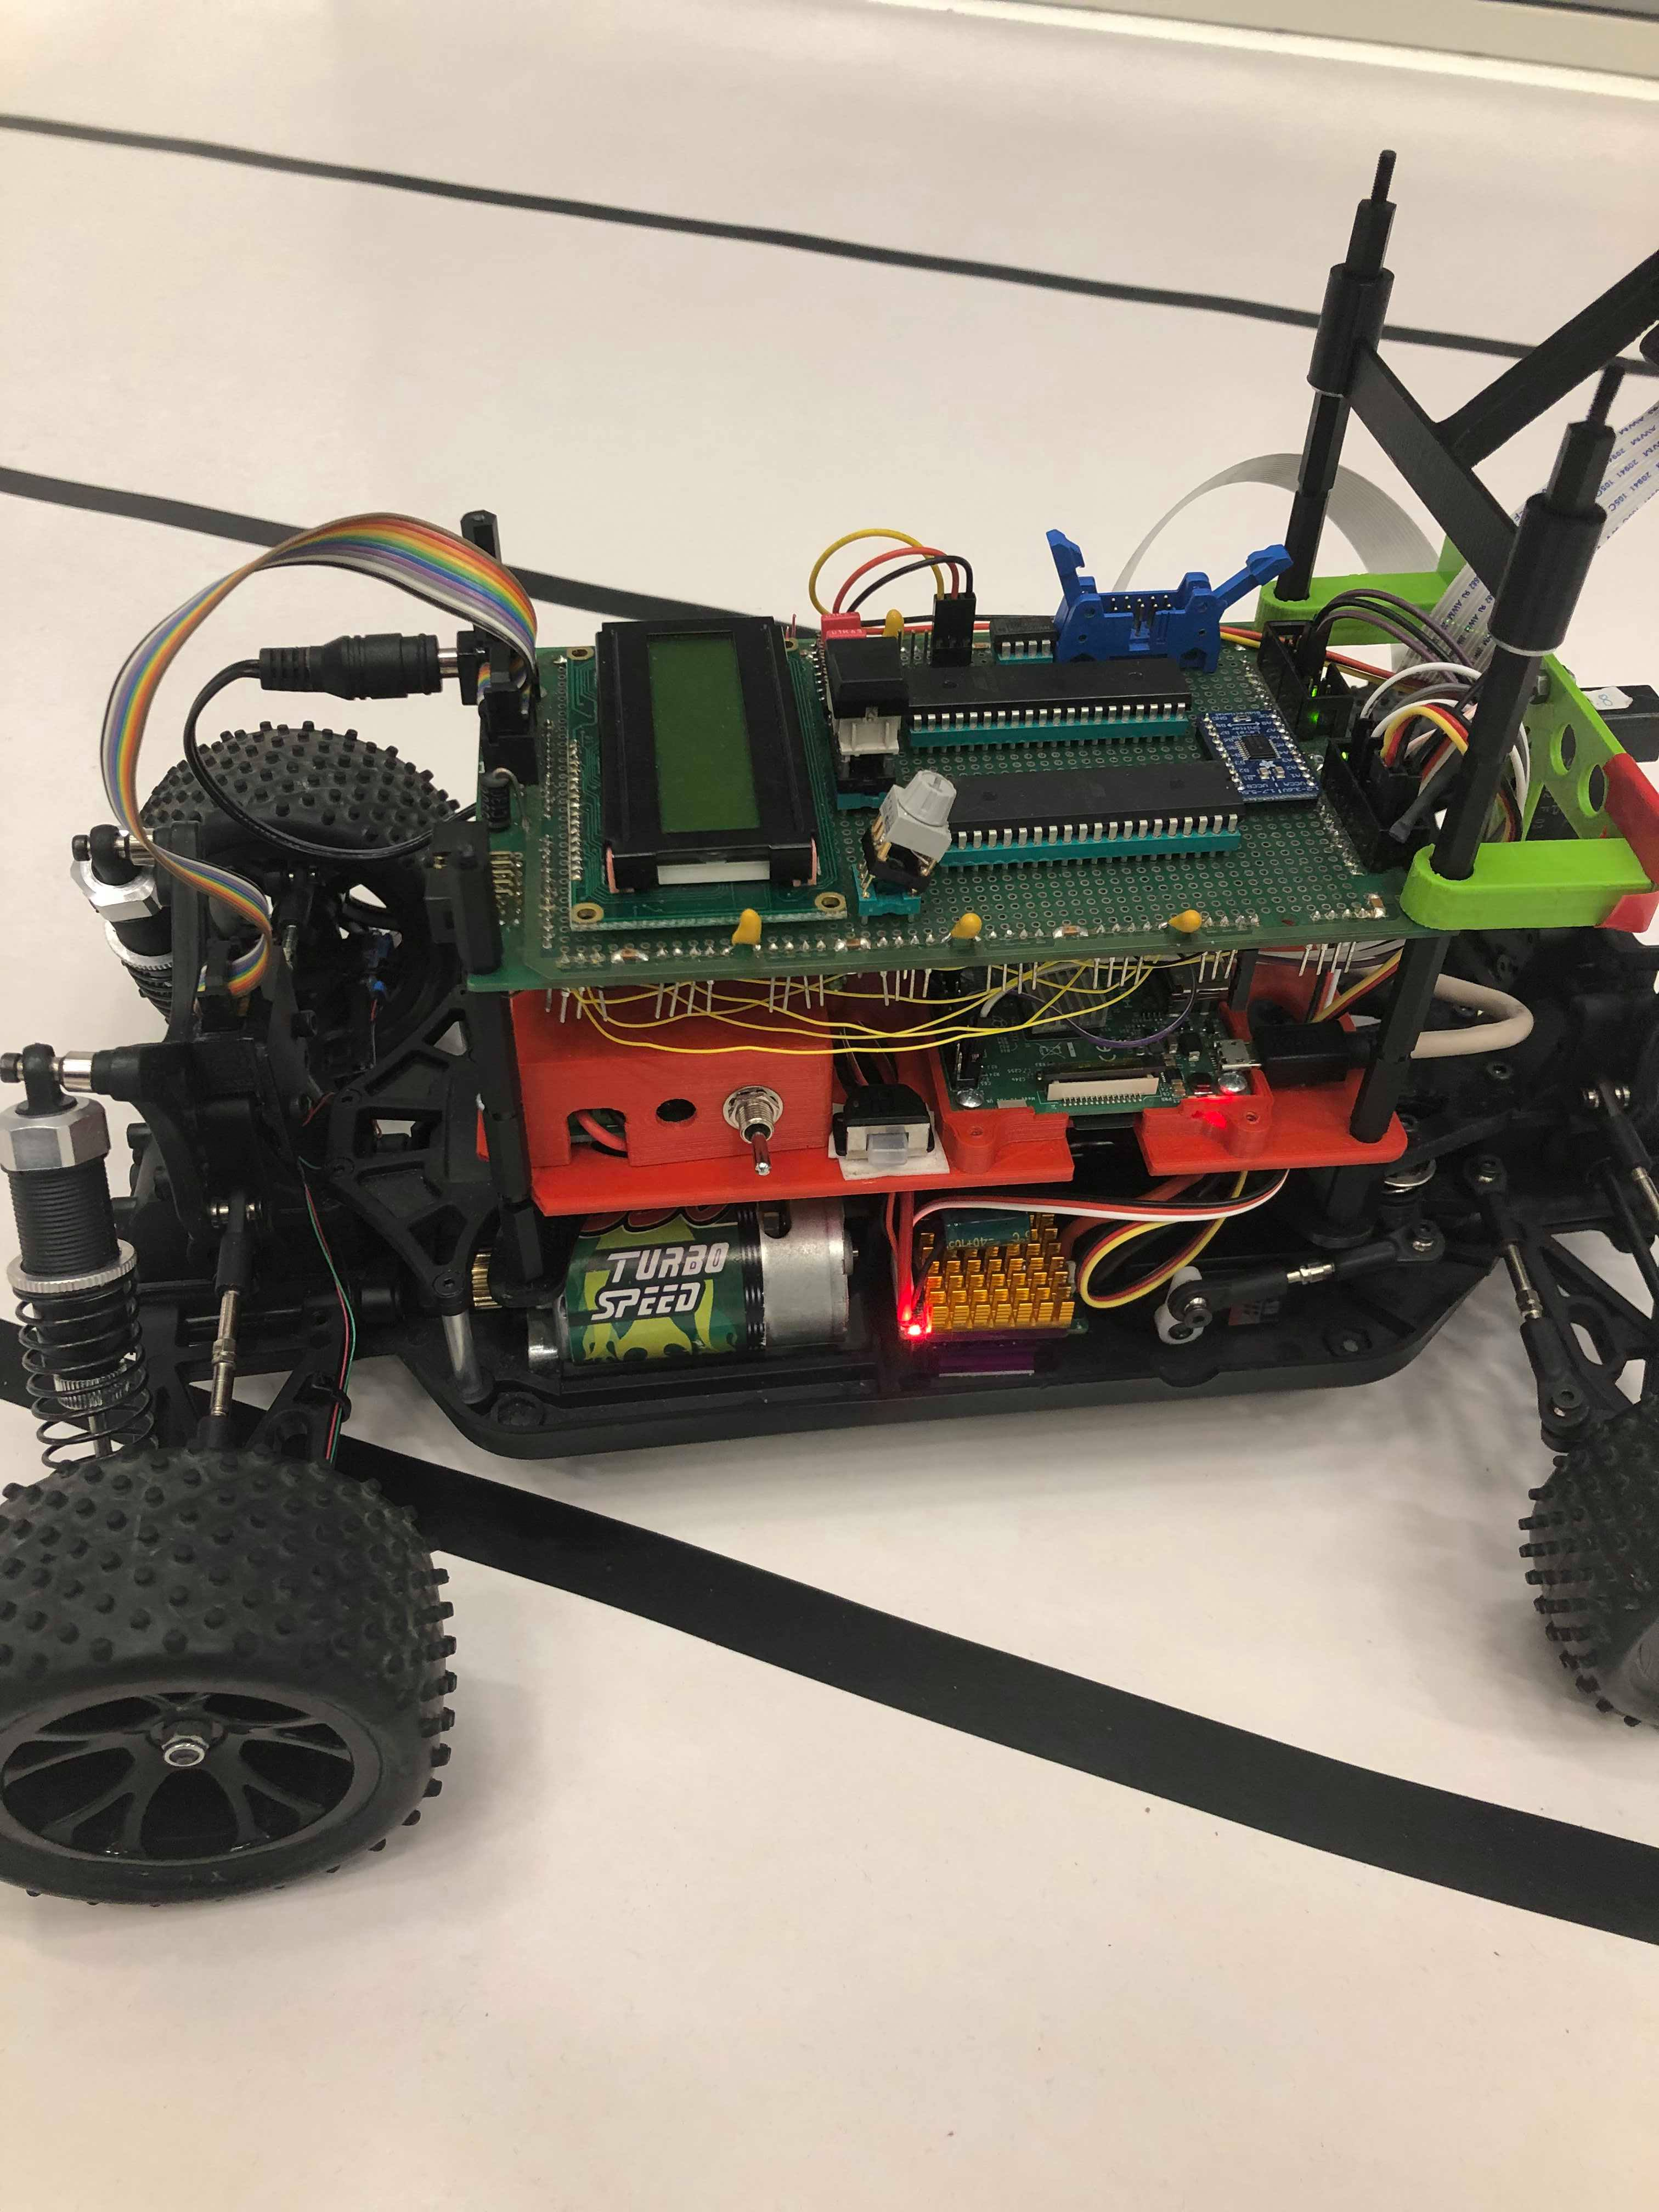
\includegraphics[width=0.6\linewidth]{\figures/bil.jpg}
    \caption{Bilen sedd från sidan där strömbrytaren för regulatorn syns, knapp
    för att starta motorn samt en reset-knapp på virkortet ovanför bilen.}
    \label{fig:sys_menu}
\end{figure}

\begin{figure}[H]
    \centering
    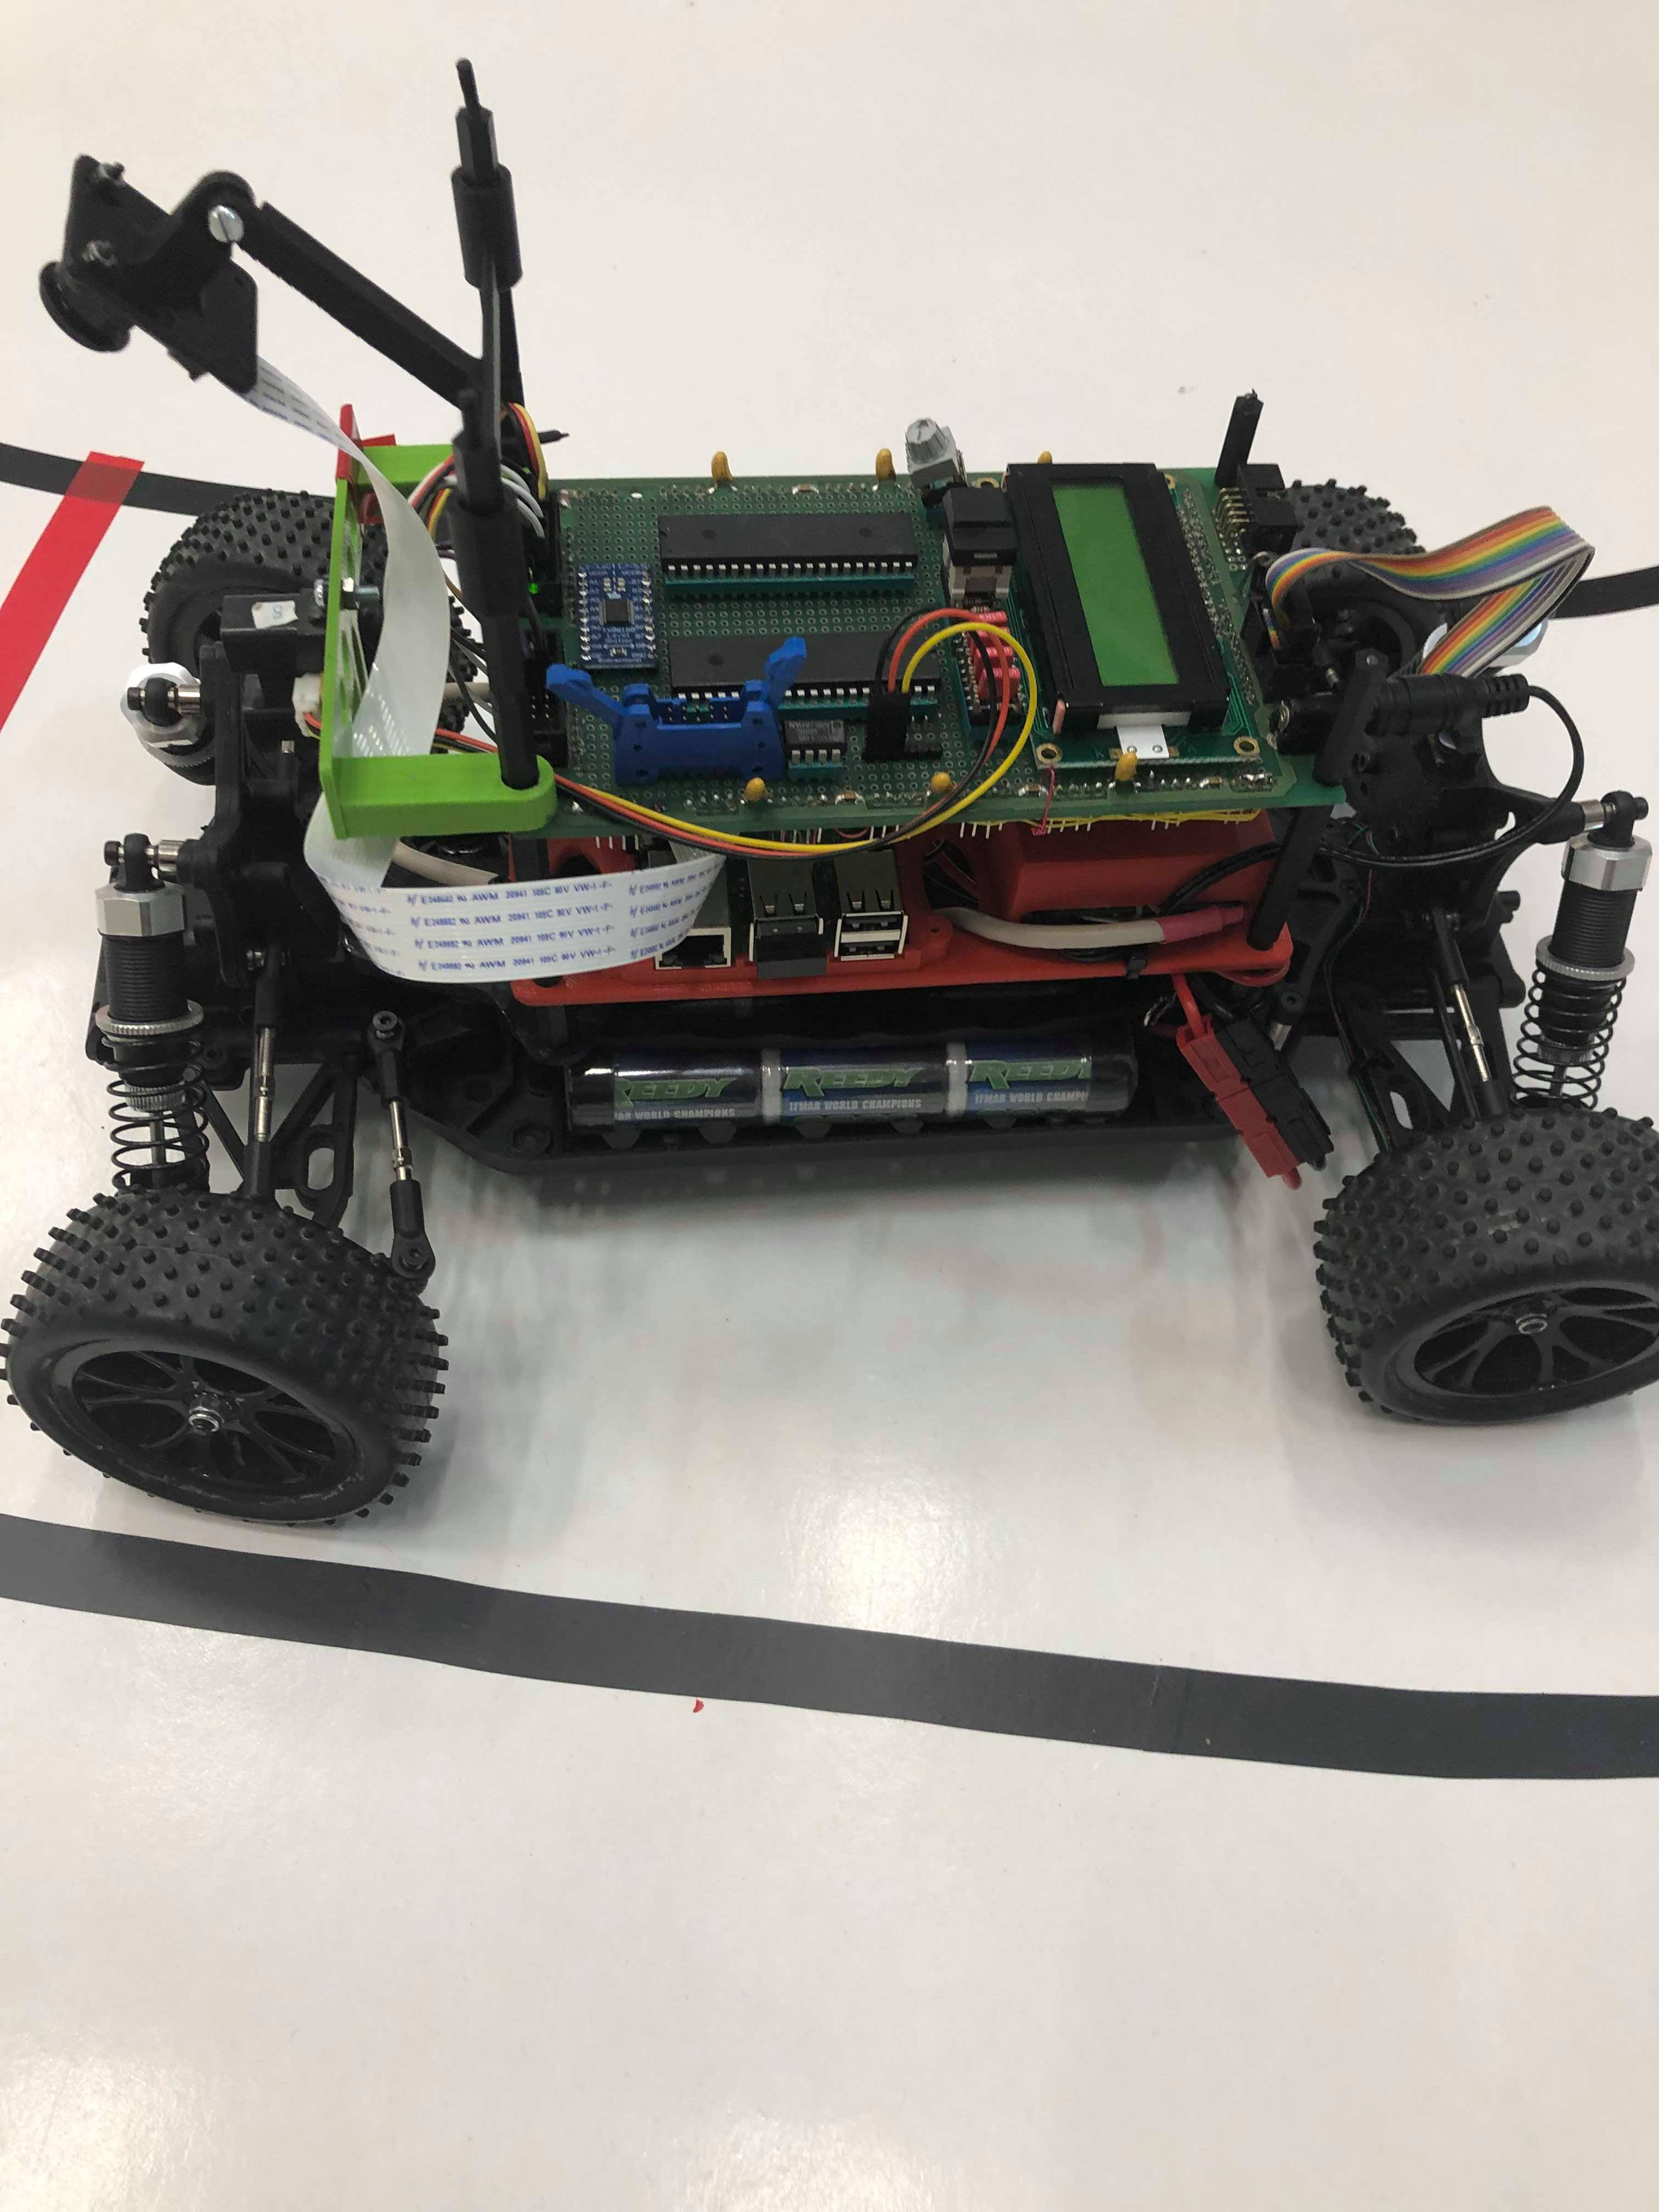
\includegraphics[width=0.6\linewidth]{\figures/bilenbatteri.jpg}
    \caption{Bilen sedd från andra sidan där batteriet är synligt längst ner på
    bilens chassi.}
    \label{fig:sys_menu}
\end{figure}

\begin{figure}[H]
    \centering
    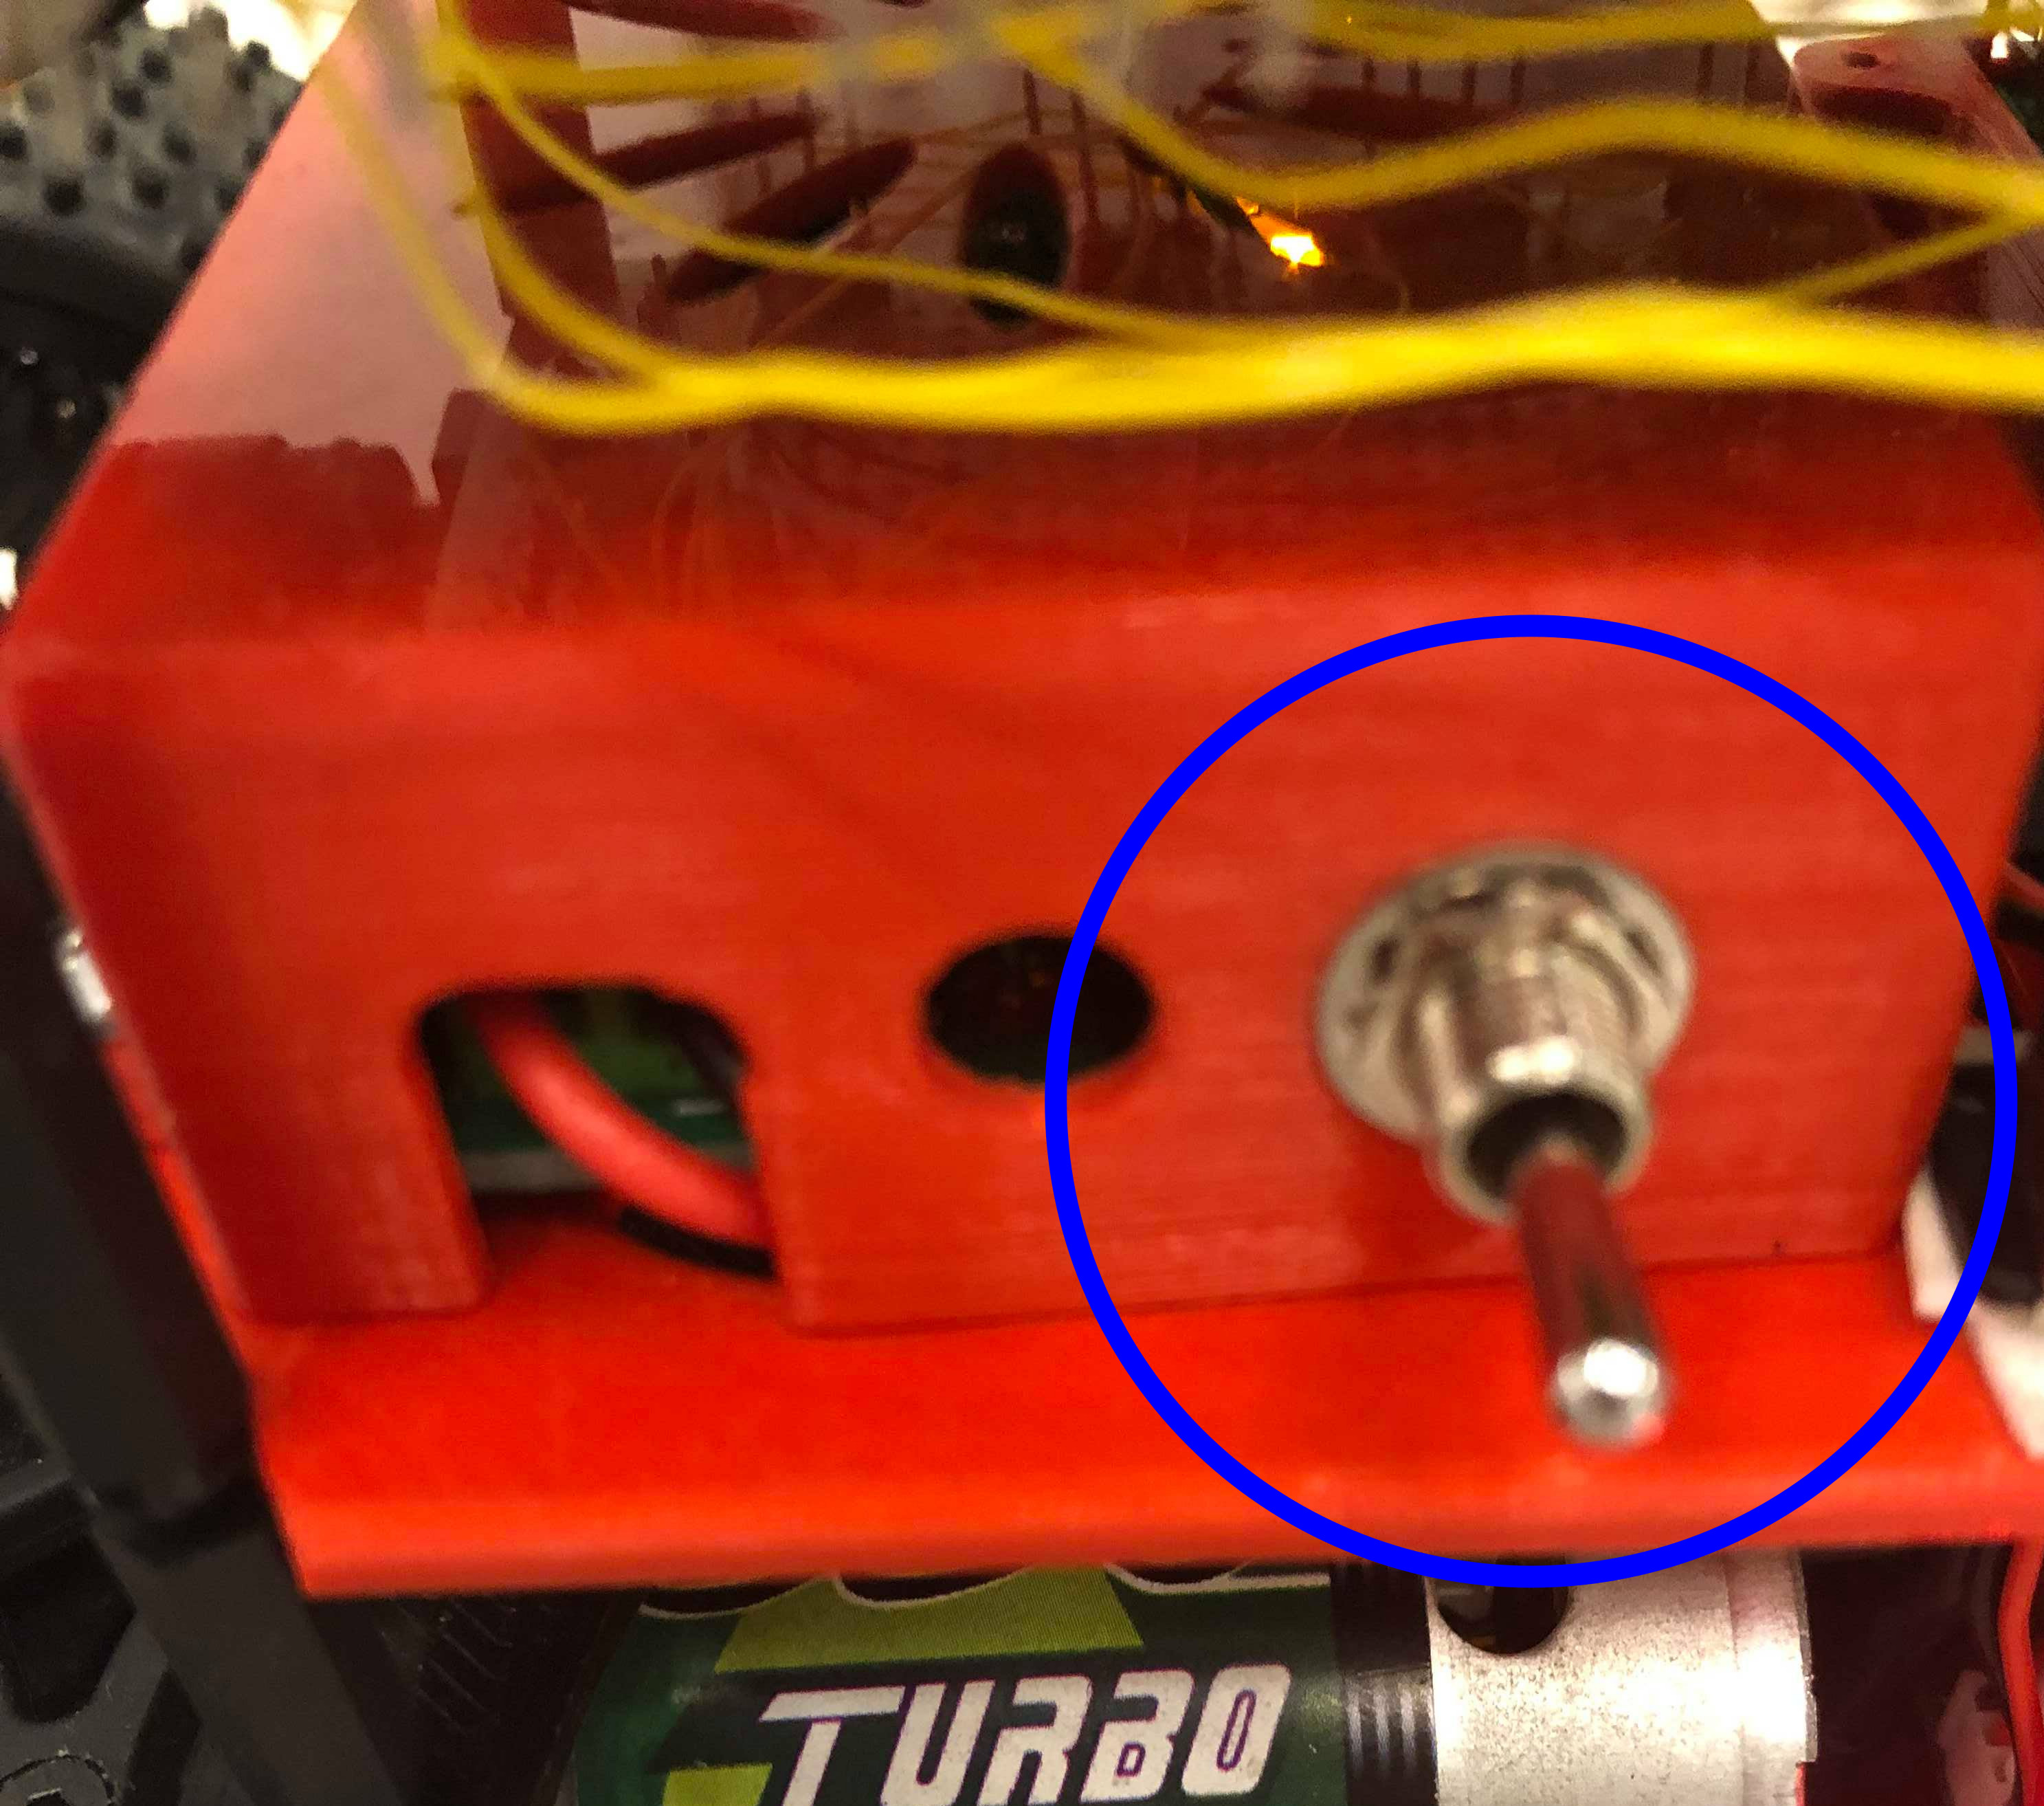
\includegraphics[width=0.6\linewidth]{\figures/switch.png}
    \caption{För att kunna starta bilen och ge övriga moduler ström måste
    strömbrytaren för spänningsregulatorn tryckas igång genom att dra spaken
    uppåt.}
    \label{fig:sys_menu}
\end{figure}

\begin{figure}[H]
    \centering
    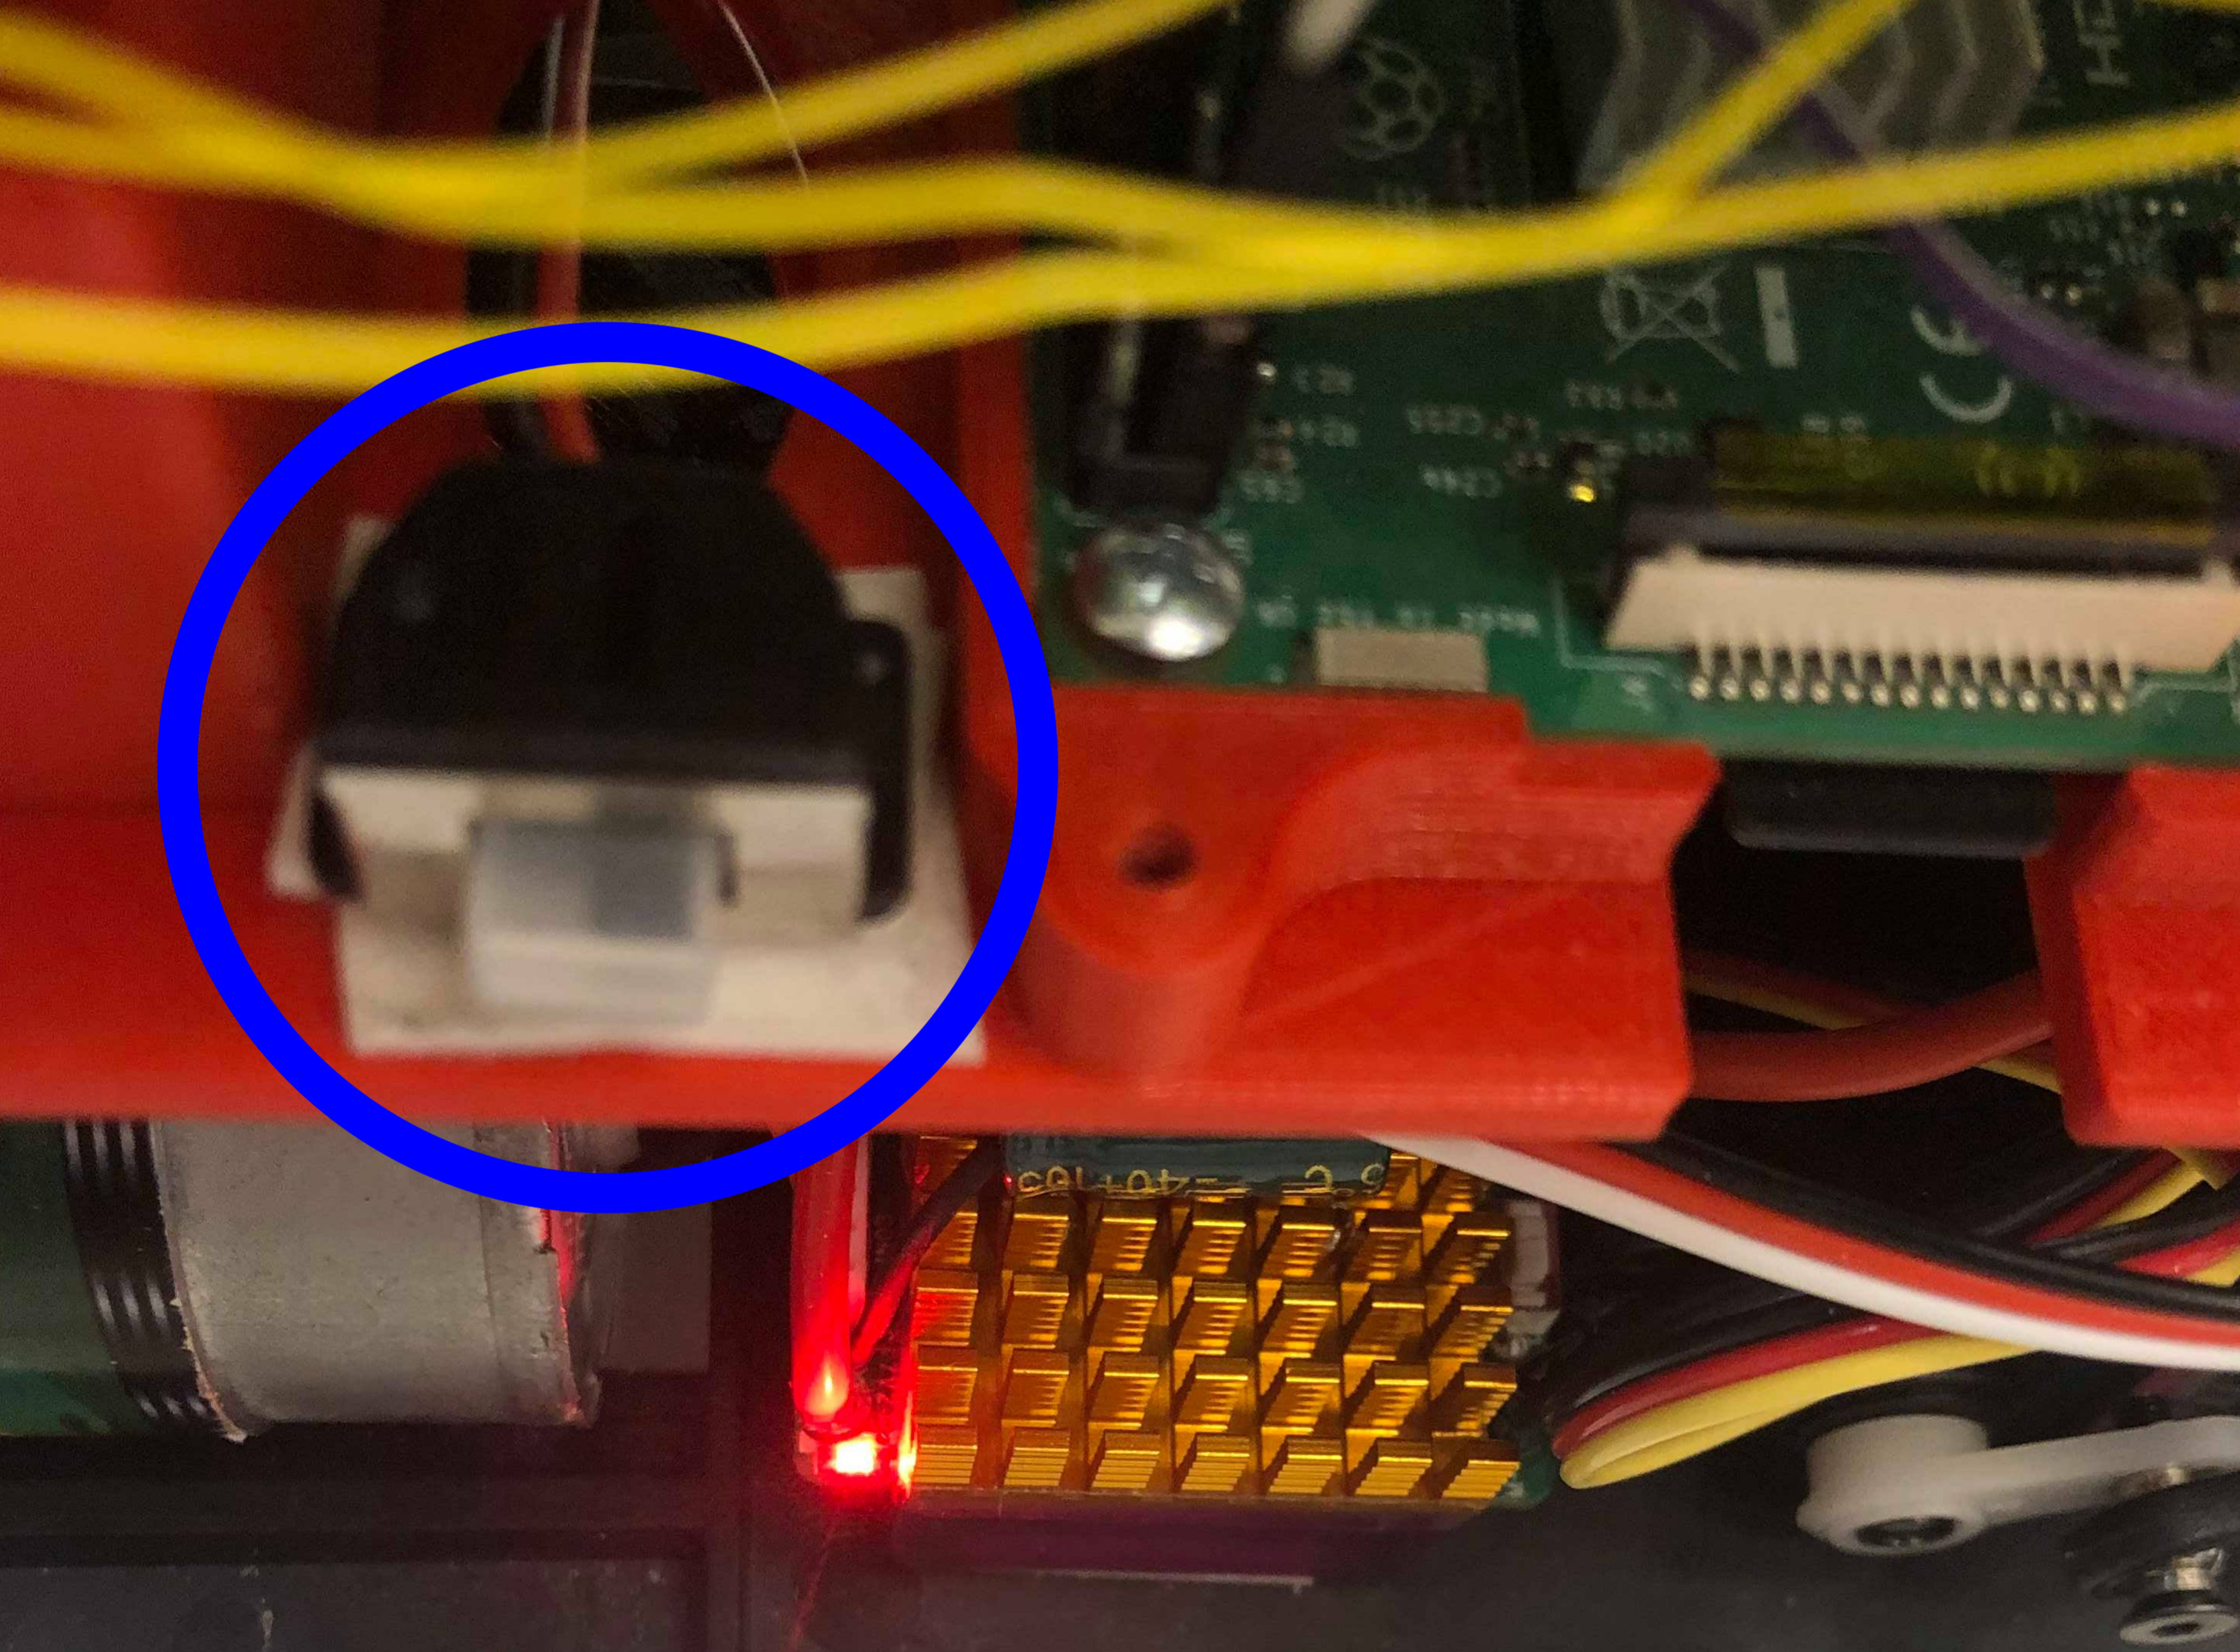
\includegraphics[width=0.6\linewidth]{\figures/motorknapp.png}
    \caption{För att starta motorn måste man trycka motorknappen till höger som
    på bilden. Tvärtom för att stänga av motorn..}
    \label{fig:sys_menu}
\end{figure}

\begin{figure}[H]
    \centering
    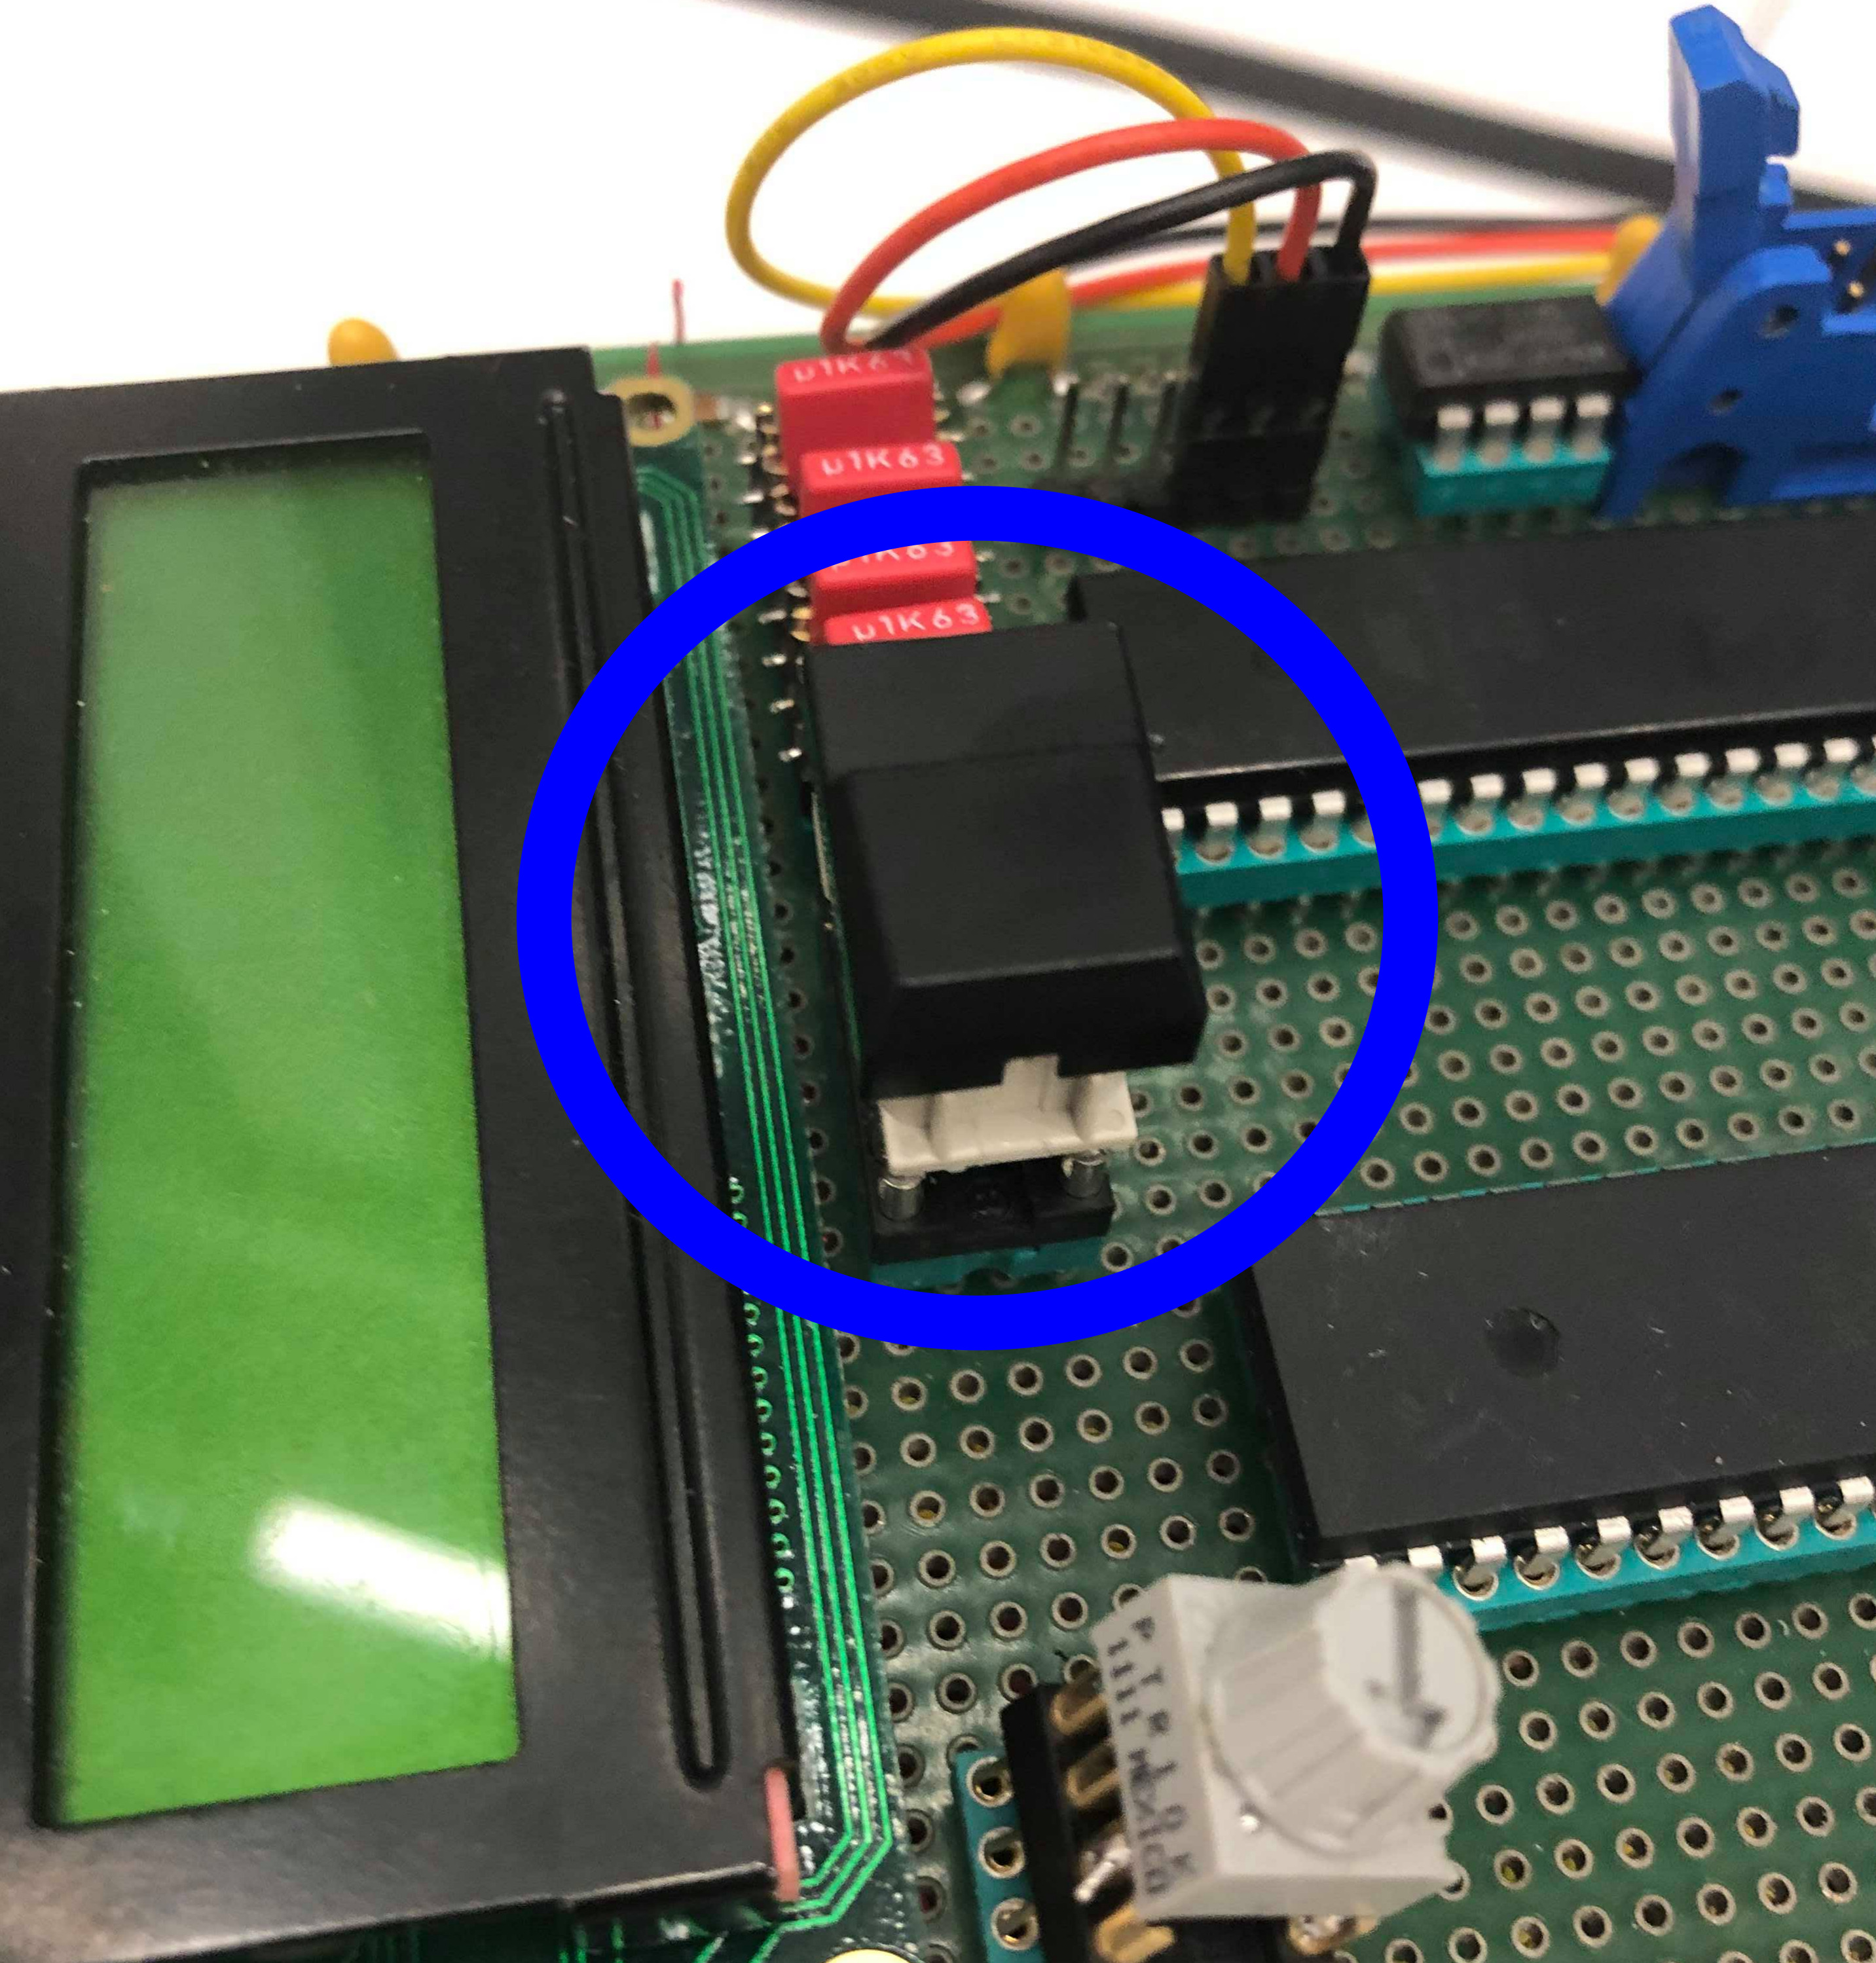
\includegraphics[width=0.6\linewidth]{\figures/reset.png}
    \caption{Reset knappen är den svarta knappen som vid nedtryckning
    återställer mikroprocessorernas värden. Bredvid till vänster ser vi
    LCD-displayen för mätvärden. }
    \label{fig:sys_menu}
\end{figure}

\begin{figure}[H]
    \centering
    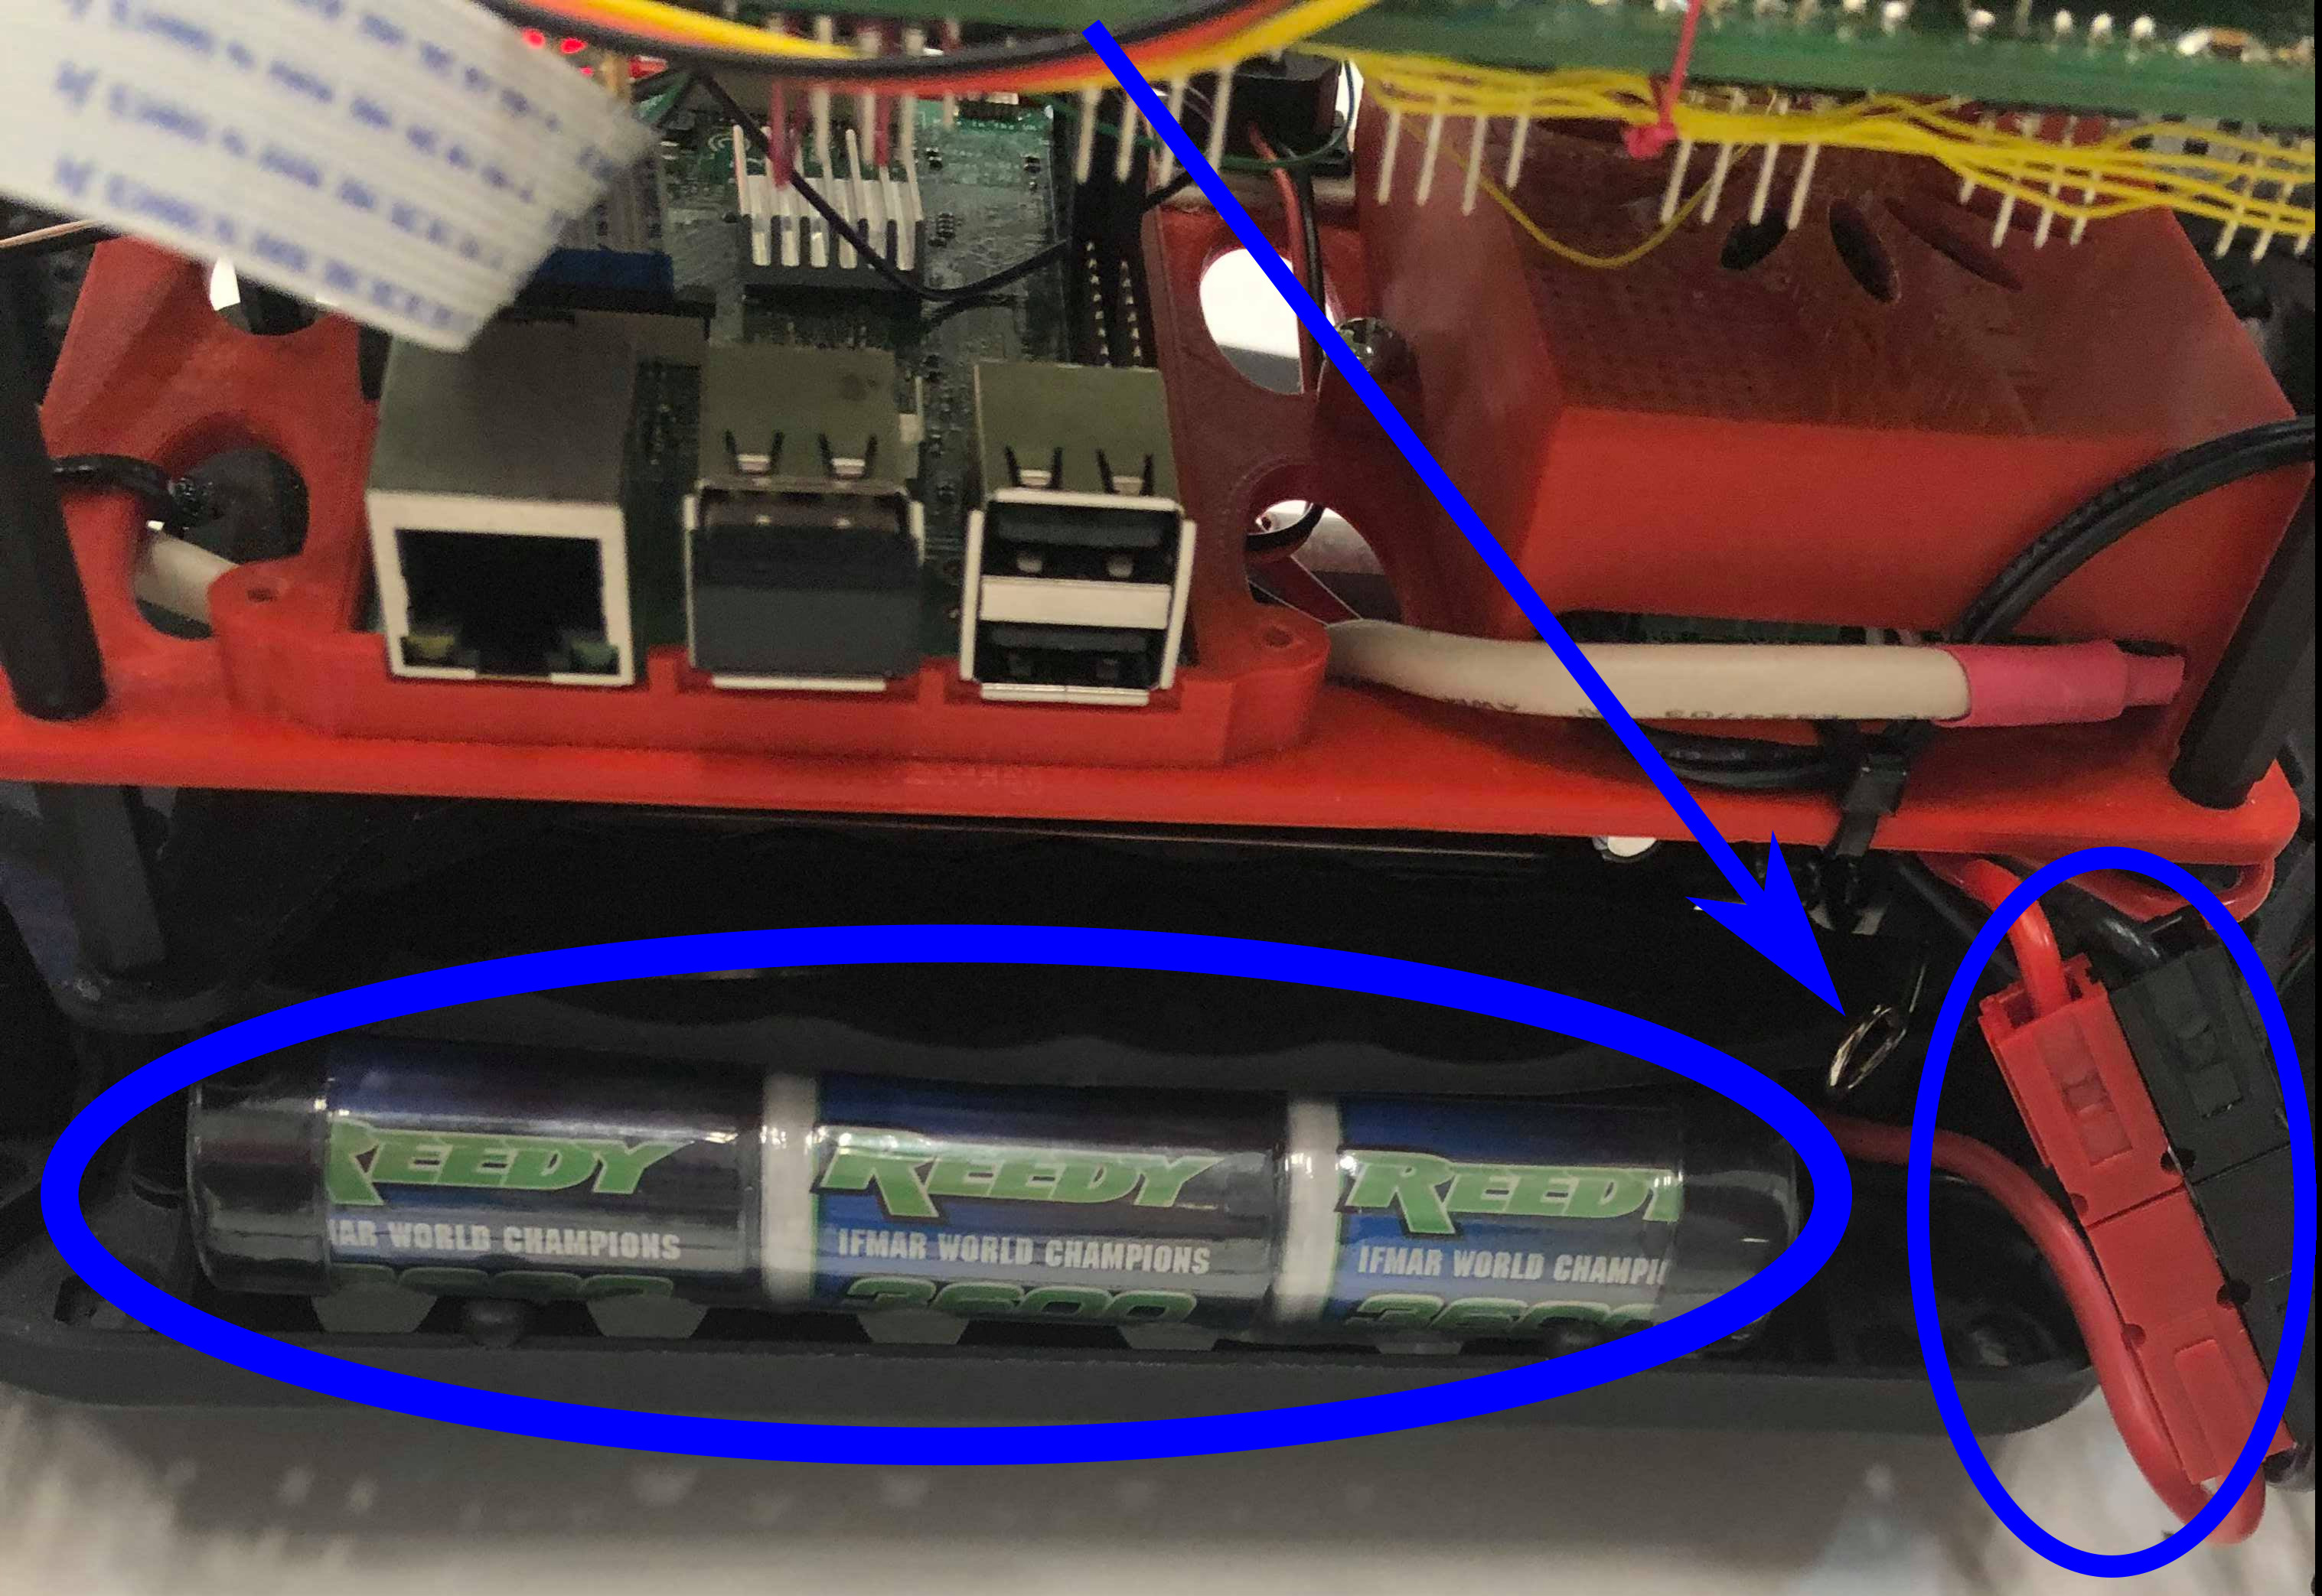
\includegraphics[width=0.6\linewidth]{\figures/batteri.png}
    \caption{För att byta batteriet måste man ta ut hårnålssprinten som pilen
    pekar på i bilden ovan. När sprinten är borta kan man dra ut kontakten till
    höger om batteriet.}
    \label{fig:sys_menu}
\end{figure}
